\documentclass[11pt]{article}
\usepackage[textwidth=18.0cm, textheight=23.0cm, top=2.0cm]{geometry}
\usepackage{pst-all}
\usepackage{amssymb}
\usepackage{tikz}
\usepackage{underscore}\begin{document}
\pagestyle{empty}


ClassName: \underline{\textbf{Class_08.2bp-6}}
\par
BinSize: \underline{\textbf{100 × 100}}
\par
ReduceSize: \underline{\textbf{100 × 100}}
\par
TypeNum: \underline{\textbf{20}}
\par
Num: \underline{\textbf{20}}
\par
OutS: \underline{\textbf{50000}}
\par
InS: \underline{\textbf{33854}}
\par
Rate: \underline{\textbf{0.677}}
\par
UB: \underline{\textbf{5}}
\par
LB0: \underline{\textbf{5}}
\par
LB: \underline{\textbf{5}}
\par
LBWithCut: \underline{\textbf{5}}
\par
NodeCut: \underline{\textbf{0}}
\par
ExtendedNodeCnt: \underline{\textbf{1}}
\par
GenNodeCnt: \underline{\textbf{1}}
\par
PrimalNode: \underline{\textbf{0}}
\par
ColumnCount: \underline{\textbf{5}}
\par
TotalCutCount: \underline{\textbf{0}}
\par
RootCutCount: \underline{\textbf{0}}
\par
LPSolverCnt: \underline{\textbf{1}}
\par
PricingSolverCnt: \underline{\textbf{0}}
\par
BranchAndBoundNum: \underline{\textbf{1}}
\par
isOpt: \underline{\textbf{true}}
\par
TimeOnInitSolution: \underline{\textbf{600.000 s}}
\par
TimeOnPrimal: \underline{\textbf{0.000 s}}
\par
TimeOnPricing: \underline{\textbf{0.000 s}}
\par
TimeOnRmp: \underline{\textbf{0.062 s}}
\par
TotalTime: \underline{\textbf{600.328 s}}
\par
\newpage


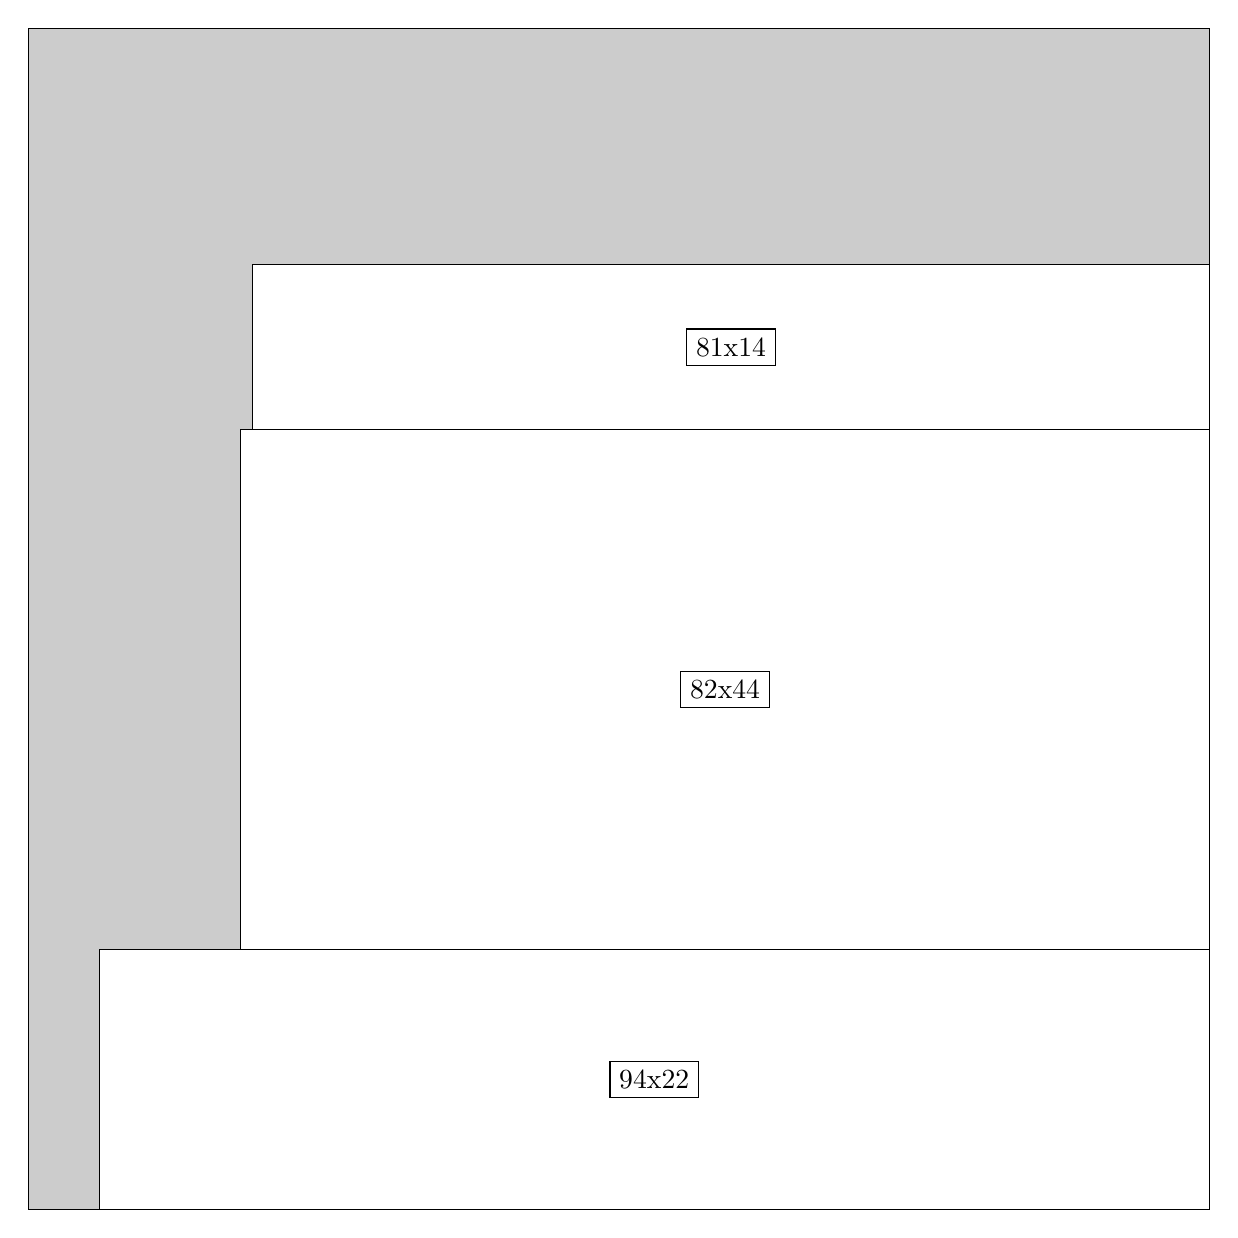
\begin{tikzpicture}[shorten >=1pt,scale=1.0,every node/.style={scale=1.0},->]
\tikzstyle{vertex}=[circle,fill=black!25,minimum size=14pt,inner sep=0pt]
\filldraw[fill=gray!40!white, draw=black] (0,0) rectangle (15.0,15.0);
\foreach \name/\x/\y/\w/\h in {94x22/0.8999999999999999/0.0/14.1/3.3,82x44/2.6999999999999997/3.3/12.299999999999999/6.6,81x14/2.85/9.9/12.15/2.1}
\filldraw[fill=white!40!white, draw=black] (\x,\y) rectangle node[draw] (\name) {\name} ++(\w,\h);
\end{tikzpicture}


w =94 , h =22 , x =6 , y =0 , v =2068
\par
w =82 , h =44 , x =18 , y =22 , v =3608
\par
w =81 , h =14 , x =19 , y =66 , v =1134
\par
\newpage


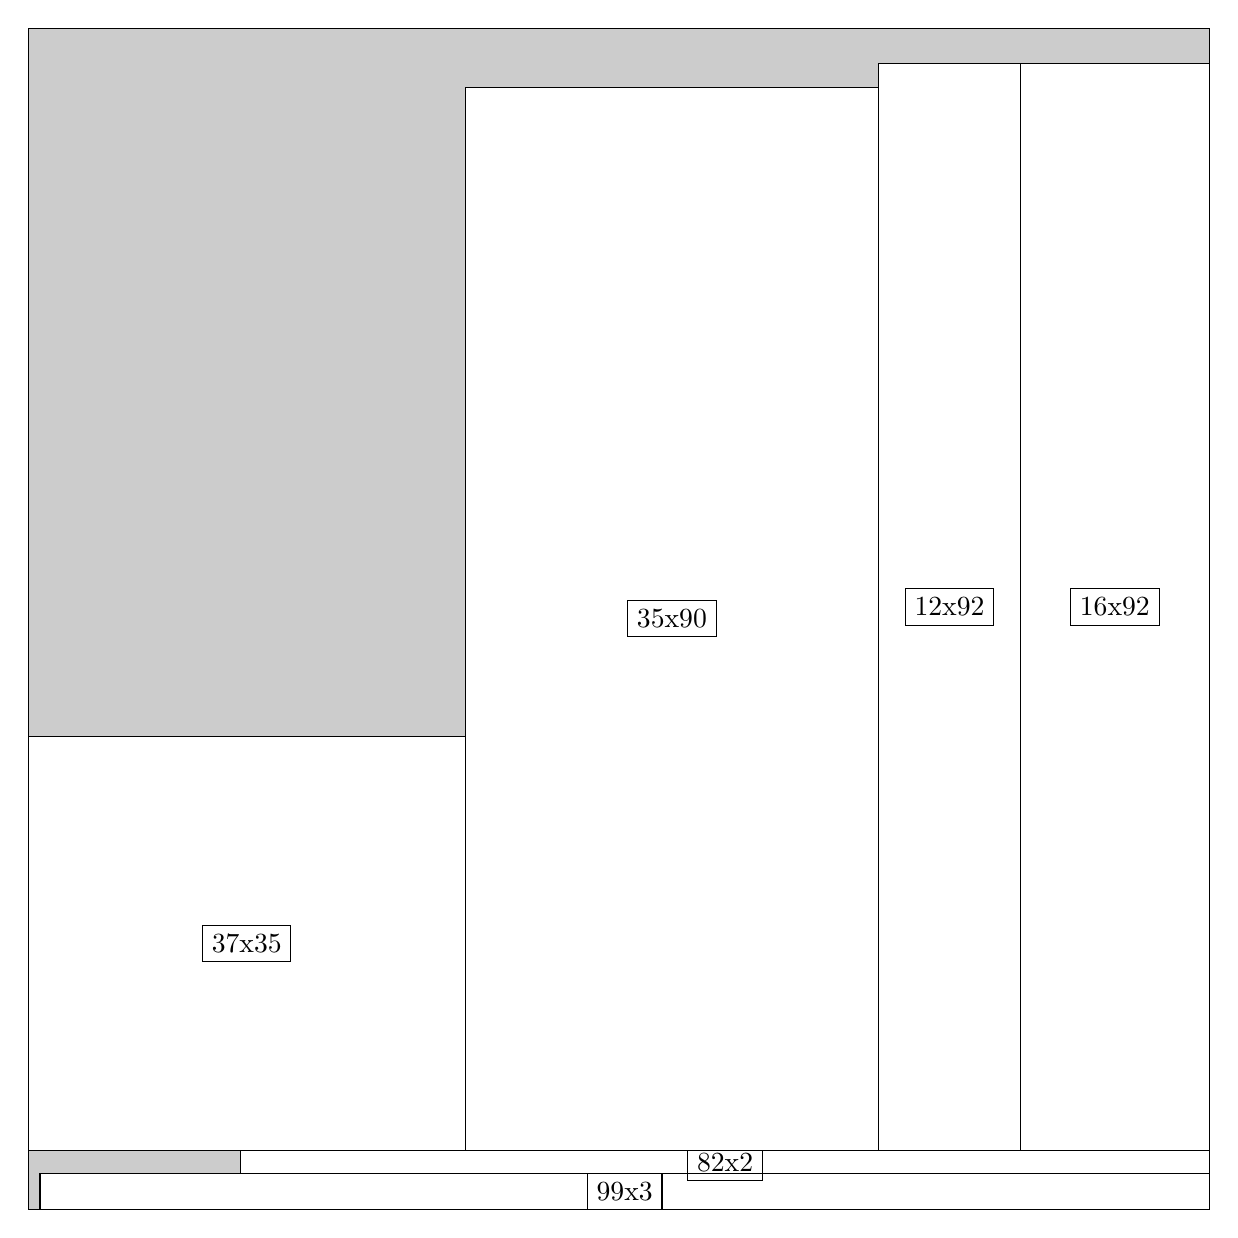
\begin{tikzpicture}[shorten >=1pt,scale=1.0,every node/.style={scale=1.0},->]
\tikzstyle{vertex}=[circle,fill=black!25,minimum size=14pt,inner sep=0pt]
\filldraw[fill=gray!40!white, draw=black] (0,0) rectangle (15.0,15.0);
\foreach \name/\x/\y/\w/\h in {99x3/0.15/0.0/14.85/0.44999999999999996,82x2/2.6999999999999997/0.44999999999999996/12.299999999999999/0.3,16x92/12.6/0.75/2.4/13.799999999999999,12x92/10.799999999999999/0.75/1.7999999999999998/13.799999999999999,35x90/5.55/0.75/5.25/13.5,37x35/0.0/0.75/5.55/5.25}
\filldraw[fill=white!40!white, draw=black] (\x,\y) rectangle node[draw] (\name) {\name} ++(\w,\h);
\end{tikzpicture}


w =99 , h =3 , x =1 , y =0 , v =297
\par
w =82 , h =2 , x =18 , y =3 , v =164
\par
w =16 , h =92 , x =84 , y =5 , v =1472
\par
w =12 , h =92 , x =72 , y =5 , v =1104
\par
w =35 , h =90 , x =37 , y =5 , v =3150
\par
w =37 , h =35 , x =0 , y =5 , v =1295
\par
\newpage


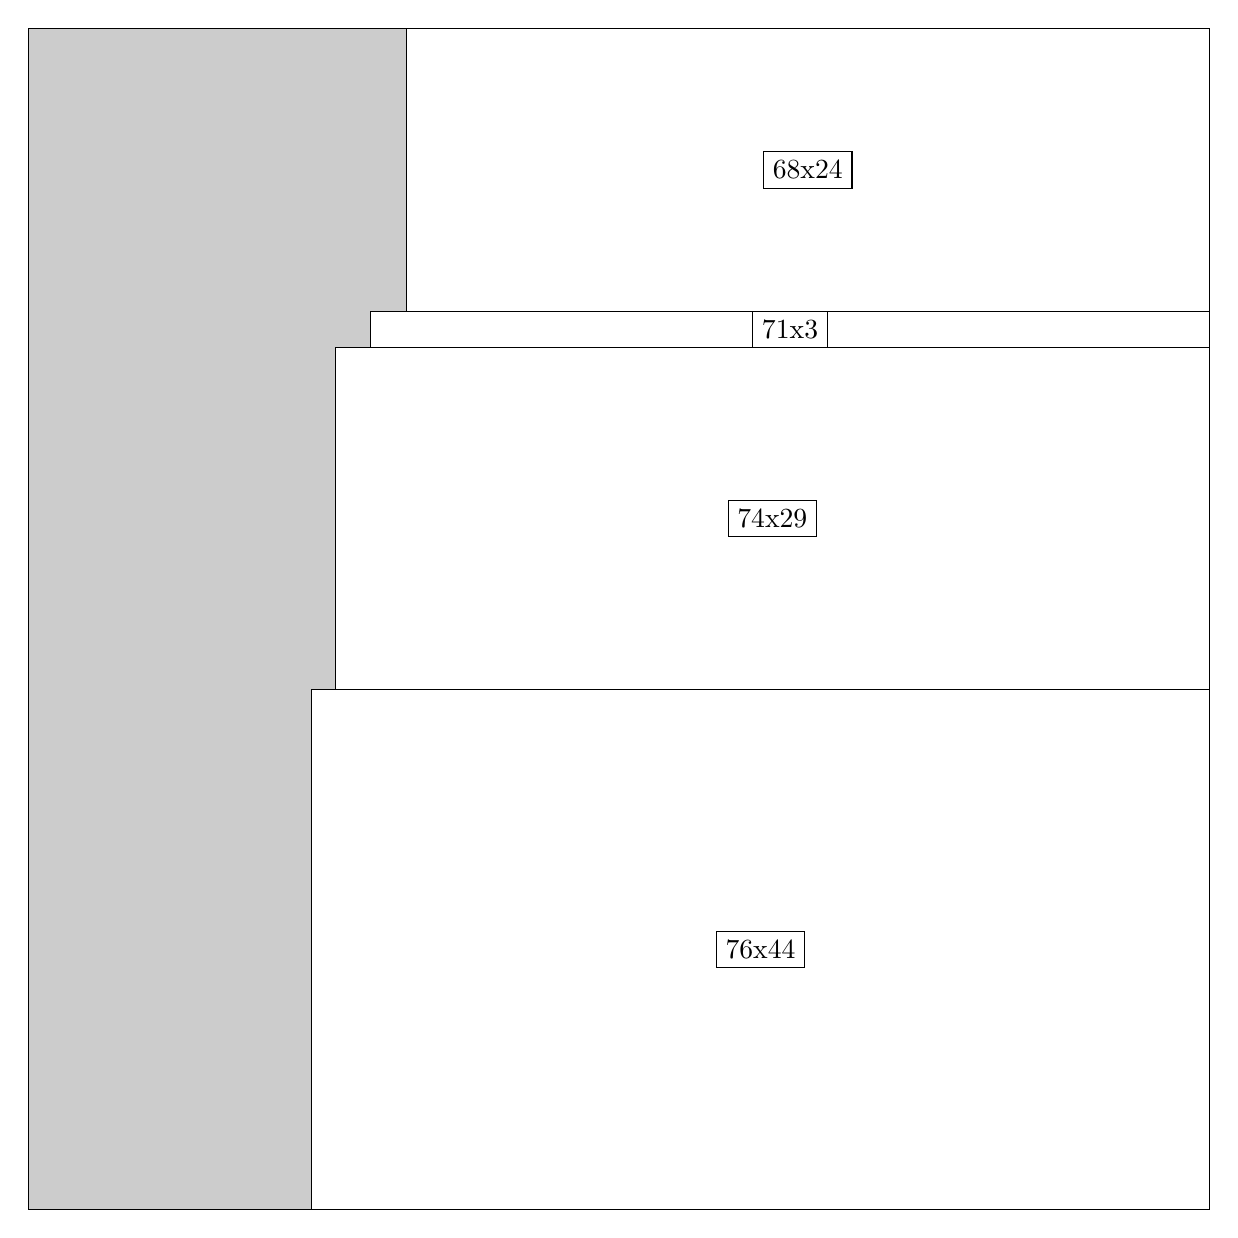
\begin{tikzpicture}[shorten >=1pt,scale=1.0,every node/.style={scale=1.0},->]
\tikzstyle{vertex}=[circle,fill=black!25,minimum size=14pt,inner sep=0pt]
\filldraw[fill=gray!40!white, draw=black] (0,0) rectangle (15.0,15.0);
\foreach \name/\x/\y/\w/\h in {76x44/3.5999999999999996/0.0/11.4/6.6,74x29/3.9/6.6/11.1/4.35,71x3/4.35/10.95/10.65/0.44999999999999996,68x24/4.8/11.4/10.2/3.5999999999999996}
\filldraw[fill=white!40!white, draw=black] (\x,\y) rectangle node[draw] (\name) {\name} ++(\w,\h);
\end{tikzpicture}


w =76 , h =44 , x =24 , y =0 , v =3344
\par
w =74 , h =29 , x =26 , y =44 , v =2146
\par
w =71 , h =3 , x =29 , y =73 , v =213
\par
w =68 , h =24 , x =32 , y =76 , v =1632
\par
\newpage


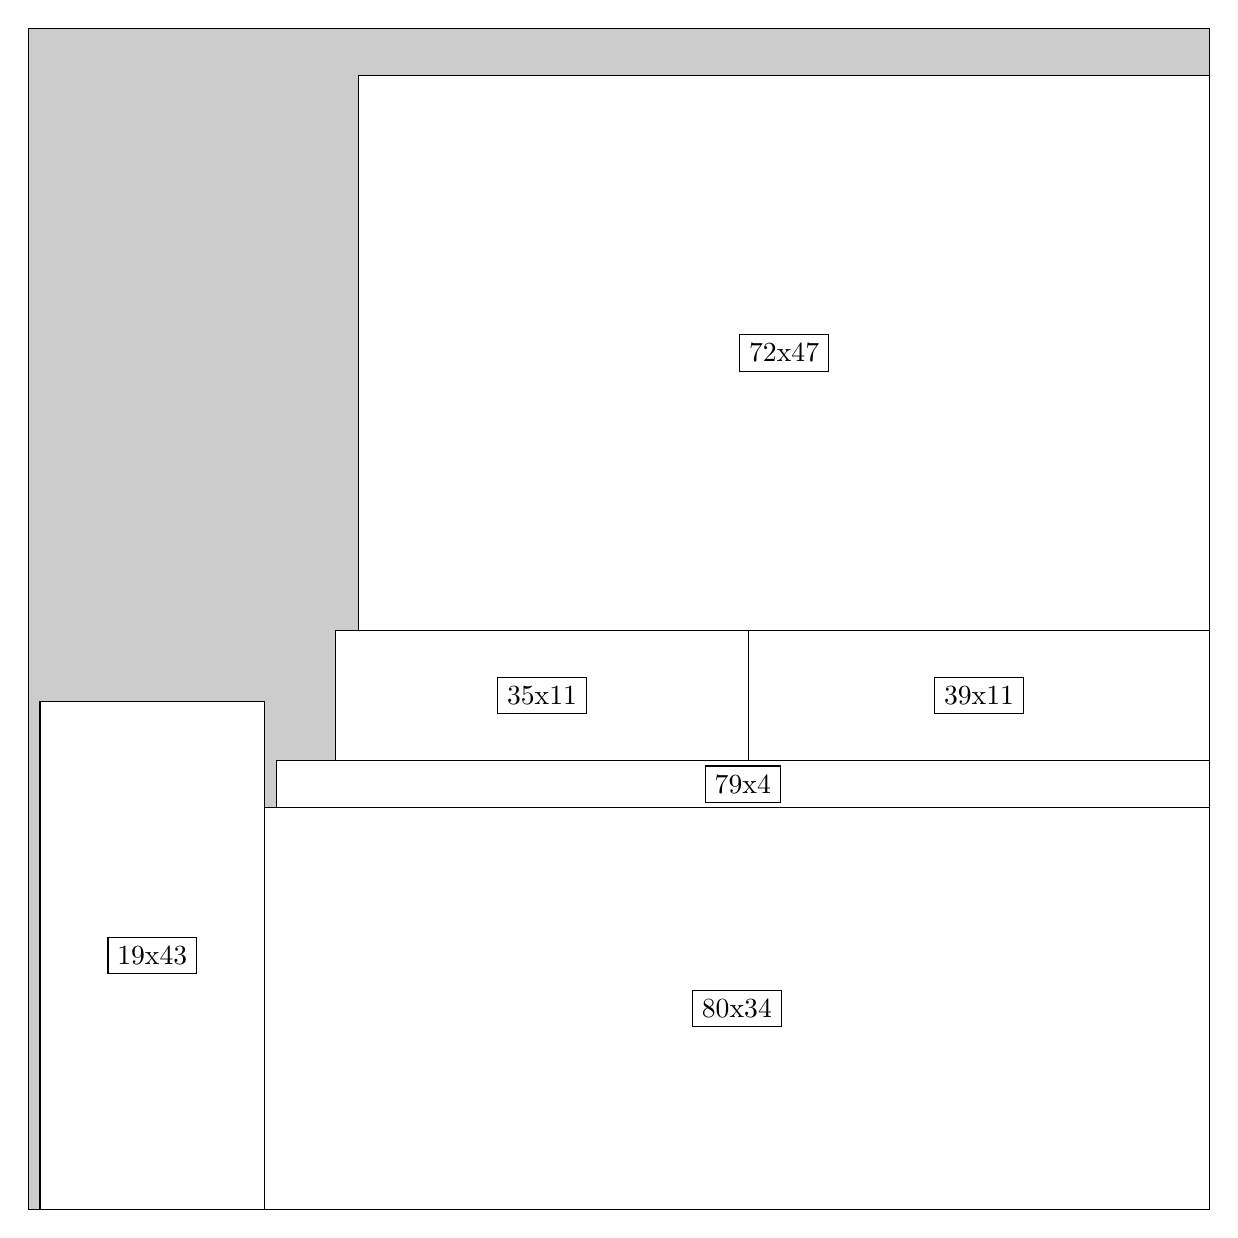
\begin{tikzpicture}[shorten >=1pt,scale=1.0,every node/.style={scale=1.0},->]
\tikzstyle{vertex}=[circle,fill=black!25,minimum size=14pt,inner sep=0pt]
\filldraw[fill=gray!40!white, draw=black] (0,0) rectangle (15.0,15.0);
\foreach \name/\x/\y/\w/\h in {80x34/3.0/0.0/12.0/5.1,79x4/3.15/5.1/11.85/0.6,39x11/9.15/5.7/5.85/1.65,35x11/3.9/5.7/5.25/1.65,72x47/4.2/7.35/10.799999999999999/7.05,19x43/0.15/0.0/2.85/6.45}
\filldraw[fill=white!40!white, draw=black] (\x,\y) rectangle node[draw] (\name) {\name} ++(\w,\h);
\end{tikzpicture}


w =80 , h =34 , x =20 , y =0 , v =2720
\par
w =79 , h =4 , x =21 , y =34 , v =316
\par
w =39 , h =11 , x =61 , y =38 , v =429
\par
w =35 , h =11 , x =26 , y =38 , v =385
\par
w =72 , h =47 , x =28 , y =49 , v =3384
\par
w =19 , h =43 , x =1 , y =0 , v =817
\par
\newpage


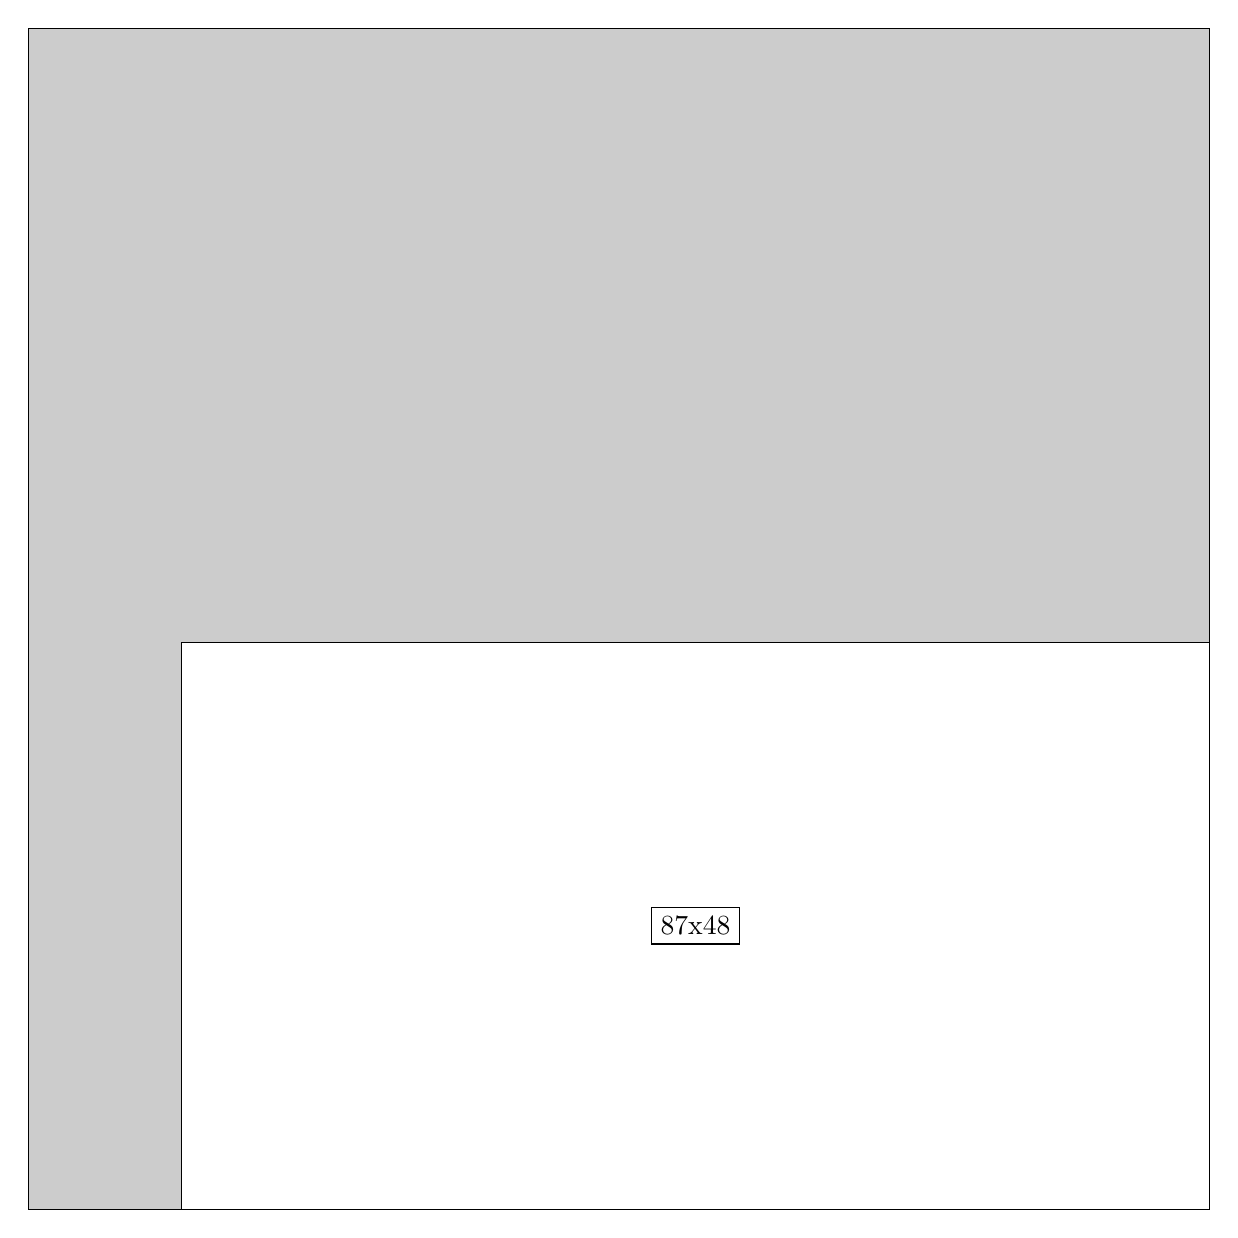
\begin{tikzpicture}[shorten >=1pt,scale=1.0,every node/.style={scale=1.0},->]
\tikzstyle{vertex}=[circle,fill=black!25,minimum size=14pt,inner sep=0pt]
\filldraw[fill=gray!40!white, draw=black] (0,0) rectangle (15.0,15.0);
\foreach \name/\x/\y/\w/\h in {87x48/1.95/0.0/13.049999999999999/7.199999999999999}
\filldraw[fill=white!40!white, draw=black] (\x,\y) rectangle node[draw] (\name) {\name} ++(\w,\h);
\end{tikzpicture}


w =87 , h =48 , x =13 , y =0 , v =4176
\par
\newpage


\end{document}